%%%%%%%%%%%%%%%%%%%%%%%%%%%%%%%%%%%%%%%%%%%%%%%%%%%%%%%%%%%%%%%%%%%%
% Authors: A. Herrera-Poyatos, F. Herrera
% Tittle: Algoritmo memético equilibrado con diversificación voraz
% 							 CAEPIA 2015
%%%%%%%%%%%%%%%%%%%%%%%%%%%%%%%%%%%%%%%%%%%%%%%%%%%%%%%%%%%%%%%%%%%%

\section{Conclusión}

	\begin{frame}{Conclusión}
		\centering
		\fontsize{8}{8}\selectfont

		{\large\textbf{Ventajas}}
		
		\kern 2mm
		\begin{tikzpicture}
			\node [fill=Grandis!80, circle,inner sep=1.5pt, text width=2cm, align=center] (ise) {Explícito e implícito};
			\node [fill=TurkishRose!80, circle,inner sep=1.5pt, text width=2cm, align=center, right= 2cm of $(ise)$] (pd) {Didáctico};
			\node [fill=ChetwodeBlue!80, circle, inner sep=1.5pt, text width=2cm, align=center, above = 16mm of $(ise)!0.5!(pd)$] (cd) {Orden 2};
			\node [fill=Jaguar!85, circle, inner sep=1.5pt, text width=2cm, align=center, below = 5mm of $(cd)$] (bd) {\color{white}{\textbf{Método del trapecio}}};
		\end{tikzpicture}

		\begin{tcolorbox}[colback=ChetwodeBlue!10,colframe=ChetwodeBlue!60]
			\large\textbf{Desventaja: existen métodos de mayor orden.}			
		\end{tcolorbox}
	\end{frame}

	\setbeamertemplate{headline}{
		\begin{beamercolorbox}[wd=\paperwidth,ht=5pt]{last head}
			
		\end{beamercolorbox}
		\begin{beamercolorbox}[sep=4pt]{title} 
			
		\end{beamercolorbox}
		\begin{beamercolorbox}[sep=4pt]{title} 
			
		\end{beamercolorbox}
	}
	\usebackgroundtemplate{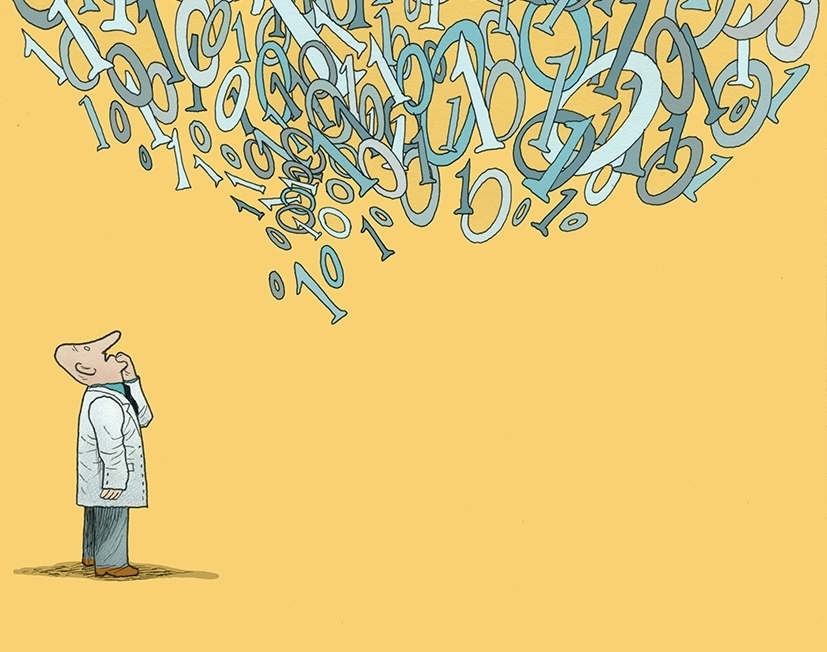
\includegraphics[height=0.9\paperheight,width=\paperwidth]{./Images/Wallpapers/BigDataCropped.jpg}}

	\begin{frame}
		\vspace{0.50\paperheight}
		\begin{titleBox}					
			\begin{beamercolorbox}[sep=2pt,center]{title}	
				\usebeamerfont{title}\textbf{Gracias por su atención.}\par
			\end{beamercolorbox}
		\end{titleBox}
		\begin{flushright}
			\fontsize{8}{8}\selectfont
			\textbf{Ilustración de Lola Moral y Sergio García}
		\end{flushright}
	\end{frame}
	